\chapter{Conclusions and future work}
%\chapter*{Concluzii}
\label{conclusions}

\section{Conclusions}
\par ASP.NET Core offers a reliable and easy choice for Web API application development. To further solidify this, the minimal API that can be created is a 4-lines long code (Figure \ref{fig:conclusions_minimal-web-api}). And, by adding the Entity Framework into the mix to take care of the database side, all that remains is the business logic.

\begin{figure}[!ht]
    \centering
    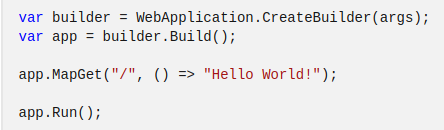
\includegraphics[width=1\linewidth]{conclusions_minimal-web-api.png}
    \caption{Minimal API with ASP.NET Core \cite{microsoftMinimalApi}}
    \label{fig:conclusions_minimal-web-api}
\end{figure}

Since React is an unopinionated library, it leaves room for a high degree of customization. But that is not without cost, since it could lead to having to reinvent the wheel and/or ending up with tons of dependencies. It's like the space-time trade-off, the best choice depends on the individuality of each project.

\section{Future work}

\subsection{Internationalization (i18n) and localization (l10n)} 

\par Internationalization (i18n) is the provisioning of the application with different languages. Internationalizing the application can expand its the reach to a global audience. Besides, since attractions could be all over the world, having the ability to switch between languages creates an easy way for comparison, which is handy for language learners.

\par Localization is the adaptation of the application to specific locales. Specifically, referring to date and time formats; number formats; symbols, icons, and colors; Right-to-Left (RTL) Language Support. This too increases the regional reach of the application.

\subsection{Accessibility (A11y)}

\par Accessibility means making the web application usable by as many people as possible, including those with disabilities. This increases the potential user base of the application.

\subsection{Responsive Design} 

\par This means making the app usable on various devices, like phones, tablets and even smart TVs. Currently the app is the design for PC/laptop screen sizes only. 

\subsection{Animations}

\par Adding animations to the application will improve the smoothness of the application and the user experience.

\subsection{Visibility for attractions}

\par Currently, only attractions collections allow setting the visibility. By extending it to attractions, it can improve the user experience by increasing the user's control of what parts of their information is publicly available. And, you can even extend the app's scope beyond the standard meaning of attractions. For example you could add your secret favorite place, even if it's not what you would normally call an attraction.

\subsection{Shared collections}

\par Are you planning a multi-destination trip with your friends/family and want to put all the suggestions or even the final itinerary in one shared place? That's where shared collections would come in.

\subsection{Personalized recommendations}
\par All the user interactions produce data: what attractions the user interacts with and how much time they spend on those attractions? what about their friends? is there a pattern to all the collections they made or to the attractions they created? etc. With collected data on such questions, an algorithm could be made that would give personalized recommendations to the users. 

\subsection{Abstracting the usage of the the UI design library}
\par Unlike the other ideas, which have in mind the user experience (UX), this is about the developer experience. The UI design library in this application (Material UI) is used as is, by directly using the components provided. But those components could be abstracted into other components, put together in one place, that only expose functionality and no implementation details of the design library. This way, should a need for the change of the UI design library appear, the required work to achieve that would be way more tedious.


\subsection{Legal and informational pages}
 \par Pages like Terms and Conditions, Privacy Policy, and Contact are crucial for regulatory compliance and for for establishing trust and transparency with users.
